\chapter{Accurate large scale modelling of Graphene Oxide}
\label{GO}
%\epigraph{``No person will deny that the highest degree of attainable accuracy is an object to be desired, and it is generally found that the last advances towards precision require a greater devotion of time, labour, and expense, than those which precede them."}{Charles Babbage}
\vspace{-9mm}
The development of accurate structures and forcefield parameters for exotic materials are paramount to the transferability of molecular dynamics investigations. Using preexisting work that posits the semi-ordered structure of graphene-oxide (GO), implemented using software developed to create semi-ordered rectangular graphene oxide sheets, we develop a bespoke forcefield using density functional theory calculations. We compare the performance of both generalised and bespoke forcefields on the behaviour of GO in solution with respect to experiments. We discover that observables diverge between generalised and bespoke forcefields in interfacial water dynamics and ion adsorption. This work provides an insight to the importance of bespoke forcefield design for combining both accuracy and scale in modelling nanomaterials at the interface. \edit{The bespoke forcefield shows strong agreement with AIMD simulations for the interfacial water dynamics and ion adsorption; we conclude that this results in the forcefield having an accuracy near that of AIMD.} \edit{Contributions for this work are as follows: \textbf{Mohamed Ali al-Badri} and \textbf{Christian D. Lorenz} conceived and planned the research. \textbf{Mohamed Ali al-Badri} and \textbf{Robert C. Sinclair} developed the nanomaterial structure software. \textbf{Mohamed Ali al-Badri} performed the calculations. \textbf{Mohamed Ali al-Badri, Paul Smith} and \textbf{Christian D. Lorenz} analysed the data and \textbf{Mohamed Ali al-Badri} prepared the final manuscript.}

%Contributions for this work are as follows: \textbf{Mohamed Ali al-Badri}: Conceptualisation, Methodology, Software, Validation, Formal analysis, Investigation, Writing - original draft, Visualisation. \textbf{Paul Smith}: Methodology, Software \edit{development for analysis scripts}, Validation, Formal analysis, Visualisation. \textbf{Robert C. Sinclair}: Methodology, Software \edit{development for creating the nanomaterial structures}. 

%addtotoc Adds an entry to the table of contents. This option requires five
%arguments, separated by commas:
%addtotoc={⟨page number ⟩,⟨section ⟩,⟨level ⟩,⟨heading ⟩,⟨label ⟩}
%⟨page number ⟩: Page number of the inserted page.
%6
%⟨section⟩: LATEX sectioning name – e.g., section, subsection, . . .
%⟨level⟩: Number, denoting depth of section – e.g., 1 for section level, 2 for
%subsection level, . . .
%⟨heading⟩: Title inserted in the table of contents.
%⟨label⟩: Name of the label. This label can be referred to with \ref and
%\pageref.



\includepdf[pages=-, offset=75 -75,addtotoc={
     1,section,1,Introduction,p1,
     2,section,1,Results,p2,
     2,subsection,2,Forcefield parameters,p2,
    %2,subsection,3,Structural fluctuations,p2,
     2,subsection,2,Water structure,p2,
    % 3,subsection,3,Interfacial water,p3,
    % 5,subsection,3,Ion adsorption,p5,
     7,section,1,Conclusions,p7,
     9,section,1,Methods,p9,
     9,subsection,2,Geometry,p9,
     9,subsection,2,Molecular Dynamics,p9,
     9,subsection,2,Density Functional Theory,p9},
     addtolist={
     3, figure,{The semi-ordered 979 atom GO sheet structure, showing regions of oxidised and unoxidised domains. Inset images highlight the structures and naming convention of aromatic carbon and alcohol, epoxy, phenol and carboxyl functional group atoms.},b,
     3, figure, {The distribution of DDEC (A) partial charge, (B) Lennard Jones $\epsilon$ and (C) Lennard Jones $\sigma$ non-bonded forcefield parameters for the component atom types of the GO sheet.OPLS parameters are presented as dashed lines.},c,
     3, figure, {The lateral illustration of OPLS and DDEC partial charges of the graphene-oxide sheet.},c,
     4,figure, {The structural deformation of the GO sheet in solution, measured by the distance from the mean in the orthogonal plane for the duration of the MD simulation for DDEC(left) and OPLS (right) forcefields.},d,
     4, table, {Mean number of intramolecular and intermolecular GO hydrogen bonds according to atom type for DDEC and OPLS GO, where the highest numbers of hydrogen bonds are highlighted. Intramolecular hydrogen bonds are normalised by the number of donor atoms. Water-GO hydrogen bonds are normalised by the number of GO atoms. Columns and rows denote accepting and donating species, respectively. Zero hydrogen bonds are denoted as dashes.}, e,
     5, figure, {The radial distribution functions of water oxygen atoms to the component GO (A) oxygen and (B) carbon atom types, according to both DDEC and OPLS forcefields and their respective hydration numbers for (C) oxygen and (D) carbon atom types.}, f,
     5, figure, {The correlation of GO atom coordination number by (A) water molecules, (B) Na$^{+}$ and (C) Cl$^{-}$ ions between the OPLS and DDEC forcefields, labeled by atom type. }, g,
     6,figure, {Intrinsic structure of the GO-water interface for both OPLS and DDEC forcefields, as indicated by (A) the intrinsic density profile, normalised to its bulk value, (B) the number of water-water hydrogen bonds ($N_{HB}$), (C) the density-weighted profile of dipole orientation ($\tilde{P}$) and (D) the density-weighted intrinsic profile of the second moment of dipole orientation ($\tilde{T}$).}, h,
     7,figure, {The joint probability density $\rho(z, \theta_{\mu})$ of the water dipole angle $\theta_{\mu}$ as a function of $z$ from the intrinsic surface of the GO sheet in solution, for both DDEC and OPLS forcefields. The difference plot shows $\rho^{\rm{DDEC}}(z, \theta_{\mu})\,-\, \rho^{\rm{OPLS}}(z, \theta_{\mu})$}, i,
     7, figure, {The radial distribution functions of sodium ions to the component GO (A) oxygen and (B) carbon atom types, according to both DDEC and OPLS forcefields and their respective mean coordination numbers for (C) oxygen and (D) carbon atom types. Error bars indicate the standard error of the mean.}, j,
     8, figure, {The radial distribution functions of chlorine ions to the component GO (A) oxygen and (B) carbon atom types, according to both DDEC and OPLS forcefields and their respective mean coordination numbers for (C) oxygen and (D) carbon atom types. Error bars indicate the standard error of the mean.}, k,
     8, table, {Adsorption half-life (ps) of ion atoms around each GO carbon type}, l,
     8, table, {Adsorption half-life (ps) of ion atoms around each GO oxygen type},m}
    ]{PDF_PAPERS/carbon_paper.pdf}      
%    ]{PDF_PAPERS/carbon_paper_fixed.pdf}      

\section*{Erratum}

    \edit{Due to an error in the plotting script, Fig.~(3.2) has been modified to accurately illustrate the distribution of OPLS and DDEC forcefield parameters. This error has no impact on the discussion, results nor other plots in the chapter. In Fig.~(\ref{fig:fixed_ddec_params} A,C), the legend colours now correctly reference the respective atom types, unlike Fig.~(3.2). The distance between the Lennard-Jones $\epsilon$ values is correctly plotted in Fig.~(\ref{fig:fixed_ddec_params} B), where previously a distribution was wrongly plotted for the DDEC values.}

\begin{figure}[ht!]
    \centering
    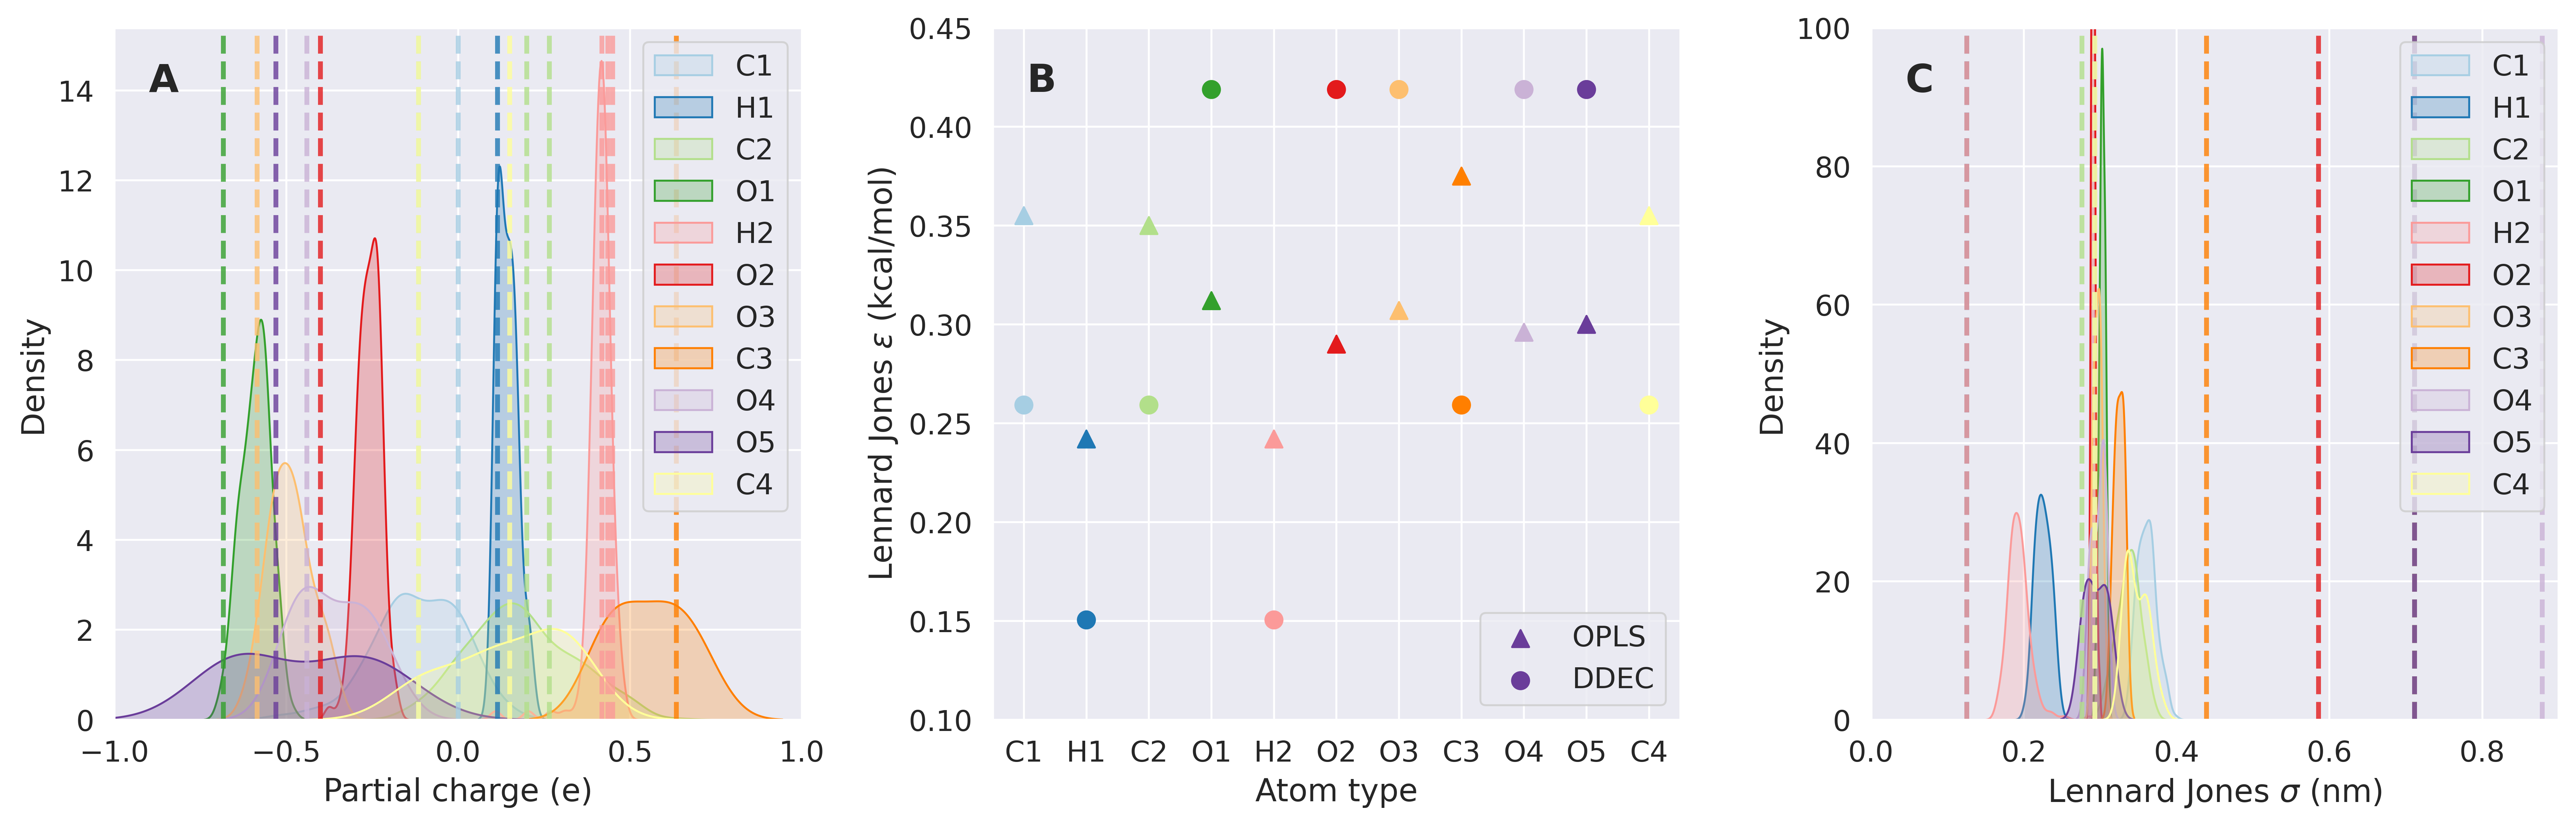
\includegraphics[width=1.0\linewidth]{ddec_params.png}
    \caption{\edit{The distribution of DDEC (A) partial charge, (B) Lennard Jones $\epsilon$ and (C) Lennard Jones $\sigma$ non-bonded forcefield parameters for the component atom types of the GO sheet. OPLS parameters are presented as dashed lines in (A) and (C), the absolute difference between the OPLS (triangle) and DDEC (circle) Lennard Jones $\epsilon$ values (gray: negative, black: positive).}}
    \label{fig:fixed_ddec_params}
\end{figure}

%addtolist={⟨page number ⟩,⟨type ⟩,⟨heading ⟩,⟨label ⟩}
%⟨page number ⟩: Page number of the inserted page.
%⟨type⟩: Name of a floating environment. (figure, table, etc.)
%⟨heading⟩: Title inserted into LoF, LoT, etc.
%⟨label⟩: Name of the label. This label can be referred to with \ref and
%\pageref.

% Actually this is a much better solution! Page command may also automatically number the pages
%
\includepdf[
%  pages=1,  offset=75 -75]{PDF_PAPERS/carbon_paper.pdf}
% \addcontentsline{toc}{section}{Introduction}
%\includepdf[
%  pages=2,
%  pagecommand=\phantomsection\addcontentsline{toc}{section}{File 02, Page 2},
%]{file_01.pdf}

%Ignore this: 
%\addcontentsline{toc}{section}{Introduction} %this will need enhanced anchoring in the respective pages
%\addcontentsline{TABLE}{LEVEL}{TITLE}
%TABLE stands for the type of list, where you want to add the item, possible are:
%
%toc: Table of contents
%lof: List of figures
%lot: List of tables
%LEVEL will be the level at which the line will appear in the list. Possible are:
%
%For toc: chapter, section, subsection
%For lof: figure
%For lot: table
%TITLE is your heading.


%\addcontentsline{lof}{figure}{Test caption!}
%
\includepdf[pages=-, offset=75 -75]{PDF_PAPERS/carbon_paper.pdf}